\section{Practical method for evaluating algorithms}\label{sec:practicalMethod}

Certain applications may require low-distortion (\eg in medical imaging), while others may prefer superior perceptual quality. How should image restoration algorithms be evaluated, then?
\begin{definition}
We say that Algorithm A \emph{dominates} Algorithm B if it has better perceptual quality \emph{and} less distortion.
\end{definition}
Note that if Algorithm A is better than B in only one of the two criteria, then neither $A$ dominates $B$ nor $B$ dominates $A$. Therefore, among a group of algorithms, there may be a large subset which can be considered equally good.
\begin{definition}
We say that an algorithm is \emph{admissible} among a group of algorithms, if it is not dominated by any other algorithm in the group.
\end{definition}
As shown in Figure~\ref{fig:dominantAdmissable}, these definitions have very simple interpretations when plotting algorithms on the perception-distortion plane. In particular, the admissible algorithms in the group, are those which lie closest to the perception-distortion bound.

\begin{figure}
	\begin{center}
		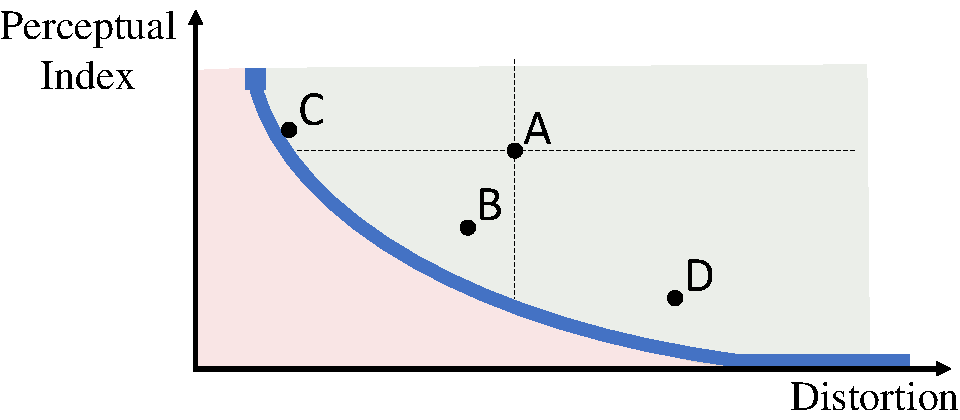
\includegraphics[width=0.85\linewidth]{figures/dominantAdmissable.pdf}
	\end{center}
	\caption{\textbf{Dominance and admissibility.} Algorithm A is dominated by Algorithm B, and is thus inadmissible. Algorithms B, C and D are all admissible, as they are not dominated by any algorithm.}
	\label{fig:dominantAdmissable}
\end{figure}

\begin{figure*}
	\begin{center}
		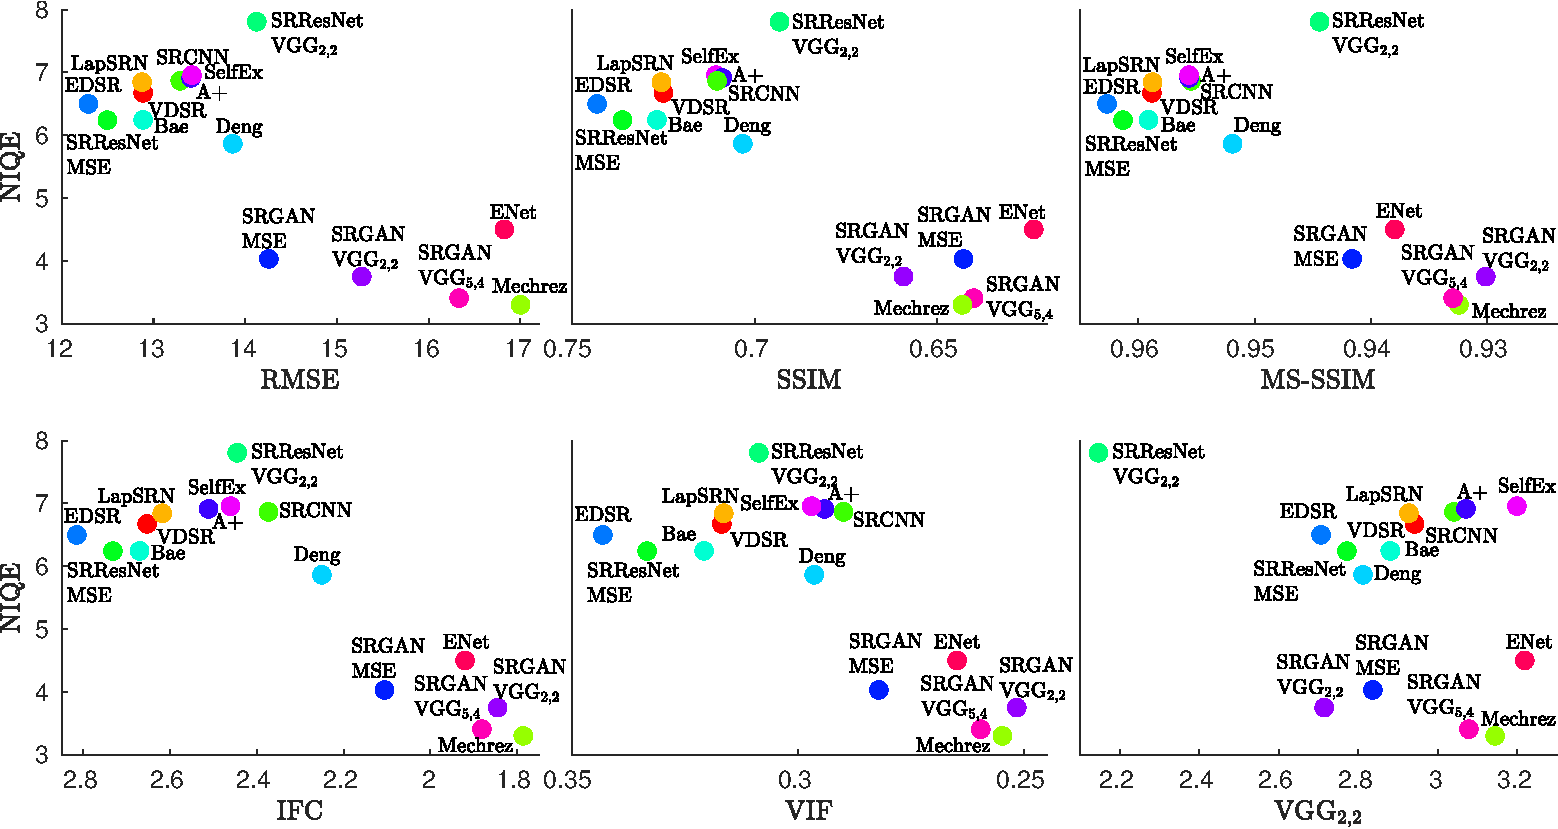
\includegraphics[width=\linewidth]{figures/NIQE.pdf}
	\end{center}
	\caption{\textbf{Perception-distortion evaluation of SR algorithms.} We plot $16$ algorithms on the perception-distortion plane. Perception is measured by the NR metric NIQE \cite{mittal2013making}. Distortion is measured by the common full-reference metrics RMSE, SSIM, MS-SSIM, IFC, VIF and VGG$_{2,2}$. In all plots, the lower left corner is blank, revealing an unattainable region in the perception-distortion plane. In proximity of the unattainable region, an improvement in perceptual quality comes at the expense of higher distortion.}
	\label{fig:noRefMethods1}
\end{figure*}

As discussed in Sec.~\ref{sec:related}, distortion is measured by \emph{full}-reference (FR) metrics, \eg \cite{wang2004image,wang2003multiscale,sheikh2005information,sheikh2006image,chandler2007vsnr,zhang2011fsim,johnson2016perceptual}. The choice of the FR metric, depends on the type of similarities we want to measure (per-pixel, semantic, etc.). Perceptual quality, on the other hand, is ideally quantified by collecting human opinion scores, which is time consuming and costly \cite{moorthy2011blind,saad2012blind}. Instead, the divergence $d(p_X,p_{\hat{X}})$ can be computed, for instance by training a discriminator net (see Sec.~\ref{sec:WGAN}). However, this requires \emph{many} training images and is thus also time consuming. A practical alternative is to utilize \emph{no}-reference (NR) metrics, \eg  \cite{mittal2012no,mittal2013making,saad2012blind,moorthy2011blind,ye2012unsupervised,kang2014convolutional,ma2017learning}, which quantify the perceptual quality of an image \emph{without} a corresponding original image. In scenarios where NR metrics are highly correlated with human mean-opinion-scores (\eg $4\times$ super-resolution \cite{ma2017learning}), they can be used as a fast and simple method for approximating the perceptual quality of an algorithm\footnote{In scenarios where NR metrics are inaccurate (\eg blind deblurring with large blurs \cite{lai2016comparative,liu2013no}), the perceptual metric should be human-opinion-scores or the loss of a discriminator trained to distinguish the algorithms' outputs from natural images.}.

\begin{figure*}
	\begin{center}
		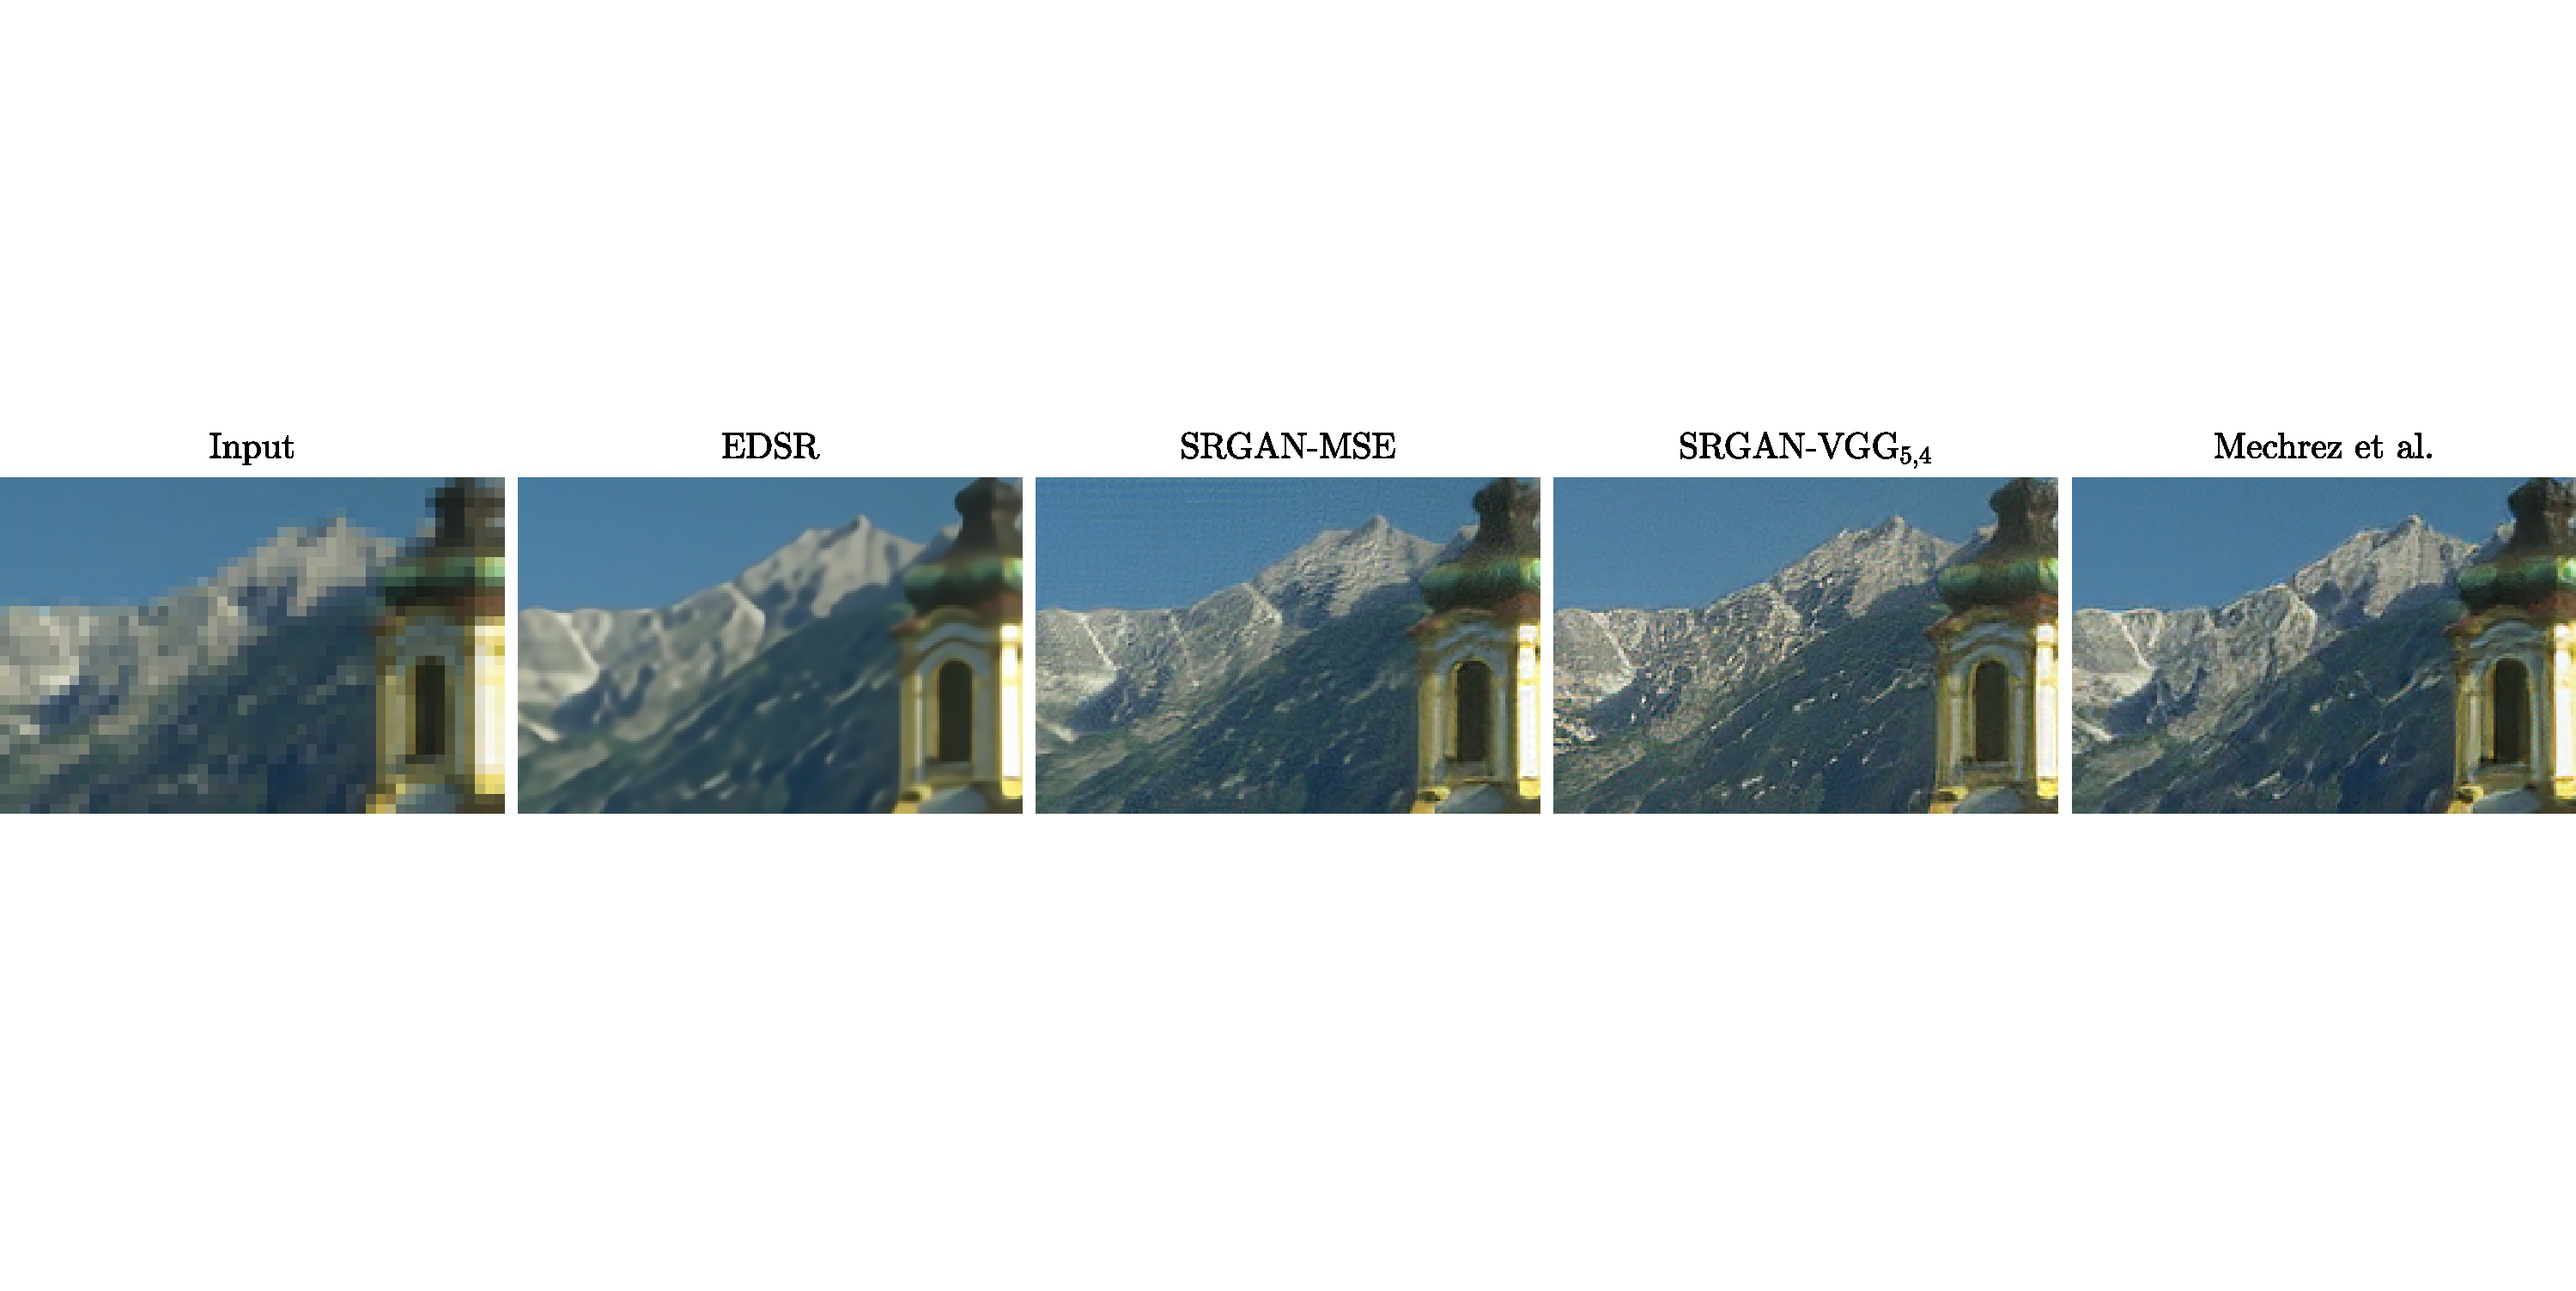
\includegraphics[width=\linewidth,trim={0 9cm 0 8.4cm},clip]{figures/church6.pdf}
	\end{center}
	\caption{\textbf{Visual comparison of algorithms closest to the perception-distortion bound.} The algorithms are ordered from low to high distortion (as evaluated by RMSE, MS-SSIM, IFC, VIF). Notice the co-occurring increase in perceptual quality.}
	\label{fig:comparison1}
\end{figure*}

We use this approach to evaluate $16$ SR algorithms in a $4\times$ magnification task, by plotting them on the perception-distortion plane (Fig.~\ref{fig:noRefMethods1}). We measure perceptual quality using the NR metric NIQE \cite{mittal2013making}, which was shown to correlate well with human opinion scores in a recent SR challenge \cite{blau2018pirm} (see Appendix \ref{sec:SR_details} for experiments with the NR metrics  BRISQUE \cite{mittal2012no}, BLIINDS-II \cite{saad2012blind} and the recent NR metric by Ma \etal \cite{ma2017learning}). We measure distortion by the five common FR metrics RMSE, SSIM \cite{wang2004image}, MS-SSIM \cite{wang2003multiscale}, IFC \cite{sheikh2005information} and VIF \cite{sheikh2006image}, and additionally by the recent $\text{VGG}_{2,2}$ metric (the distance in the feature space of a VGG net) \cite{ledig2016photo,johnson2016perceptual}. To conform to previous evaluations, we compute all metrics on the y-channel after discarding a 4-pixel border (except for VGG$_{2,2}$, which is computed on RGB images). Comparisons on color images can be found in Appendix \ref{sec:SR_details}. The algorithms are evaluated on the BSD100 dataset \cite{martin2001database}. The evaluated algorithms include: A+ \cite{timofte2014a+}, SRCNN \cite{dong2014learning}, SelfEx \cite{huang2015single}, VDSR~\cite{kim2016accurate}, Johnson \etal~\cite{johnson2016perceptual}, LapSRN \cite{lai2017deep}, Bae \etal~\cite{bae2017beyond} (``primary'' variant), EDSR \cite{lim2017enhanced}, SRResNet variants which optimize MSE and $\text{VGG}_{2,2}$ \cite{ledig2016photo}, SRGAN variants which optimize MSE, $\text{VGG}_{2,2}$, and $\text{VGG}_{5,4}$, in addition to an adversarial loss \cite{ledig2016photo}, ENet \cite{sajjadi2017enhancenet} (``PAT'' variant), Deng \cite{deng2018enhancing} ($\gamma=0.55$), and Mechrez \etal~\cite{Mechrez2018SR}.


Interestingly, the same pattern is observed in all plots:
(i) The lower left corner is blank, revealing an unattainable region in the perception-distortion plane. (ii) In proximity of this blank region, NR and FR metrics are \emph{anti-correlated}, indicating a tradeoff between perception and distortion. Notice that the tradeoff exists even for the IFC, VIF and VGG$_{2,2}$ measures, which are considered to capture visual quality better than MSE and SSIM.

Figure~\ref{fig:comparison1} depicts the outputs of several algorithms lying closest to the perception-distortion bound in the IFC graph in Fig. \ref{fig:noRefMethods1}. While the images are ordered from low to high distortion (according to IFC), their perceptual quality clearly improves from left to right.

Both FR and NR measures are commonly validated by calculating their correlation with human opinion scores, based on the assumption that both should be correlated with perceptual quality. However, as Fig.~\ref{fig:Ma_IFC_correlation} shows, while FR measures can be well-correlated with perceptual quality when distant from the unattainable region, this is clearly not the case when approaching the perception-distortion bound. In particular, all tested FR methods are inconsistent with human opinion scores which found the SRGAN to be superb in terms of perceptual quality \cite{ledig2016photo}, while NR methods successfully determine this. We conclude that image restoration algorithms should always be evaluated by a pair of NR and FR metrics, constituting a reliable, reproducible and simple method for comparison, which accounts for both perceptual quality and distortion. This evaluation method was demonstrated and validated by a human opinion study in the 2018 PIRM super-resolution challenge \cite{blau2018pirm}.

\begin{figure}
	\begin{center}
		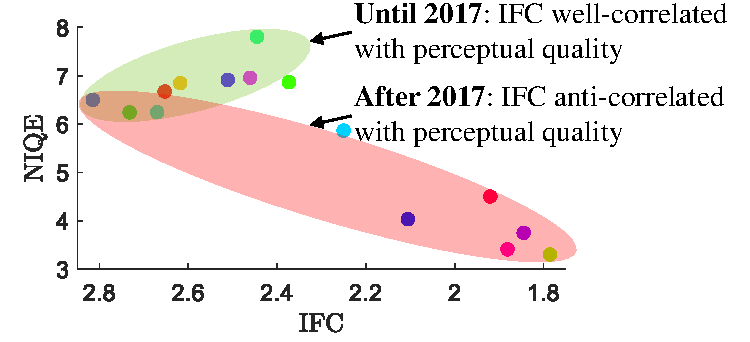
\includegraphics[width=0.95\linewidth]{figures/NIQE_IFC_corr.pdf}
	\end{center}
	\caption{\textbf{Correlation between distortion and perceptual quality.} In proximity of the perception-distortion bound, distortion and perceptual quality are \emph{anti-correlated}. However, correlation is possible at distance from the bound.}
	\label{fig:Ma_IFC_correlation}
\end{figure}


Up until 2016, SR algorithms occupied only the upper-left section of the perception-distortion plane. Nowadays, emerging techniques are exploring new regions in this plane. The SRGAN, ENet, Deng, Johnson \etal~and Mechrez \etal~methods are the first (to our knowledge) to populate the high perceptual quality region. In the near future we will most likely witness continued efforts to approach the perception-distortion bound, not only in the low-distortion region, but throughout the entire plane.
